Con il presente documento il gruppo MERL intende comunicarLe che si impegnerà a terminare il progetto didattico entro il giorno 6 Maggio 2022.

Dopo un’attenta discussione siamo riusciti a elaborare un preventivo relativo al capitolato C5 Login Warrior dell’azienda Zucchetti S.p.A.. Il gruppo ha deciso di dividersi equamente le ore di lavoro per ciascun ruolo da assumere durante svolgimeto del progetto. La seguente tabella indica le ore di lavoro dei vari ruoli che si occupano del progetto e dei loro relativi costi.

\begin{center}
  \begin{tabular}{ |l|c|c|c|c| }
    \hline
                   & Ore Ind. & Ore Totali & Costo (€/h) & Costo Totale (€) \\
    \hline
    Responsabile   & 9   & 63         & 30        & 1890             \\
    \hline
    Amministratore & 8   & 56         & 20        & 1120             \\
    \hline
    Analista       & 5   & 35         & 25        & 875              \\
    \hline
    Progettista    & 23  & 161        & 25        & 4025             \\
    \hline
    Programmatore  & 24  & 168        & 15        & 2520             \\
    \hline
    Verificatore   & 26  & 182        & 15        & 2730             \\
    \hline
  \end{tabular}
\end{center}

Di seguito riportiamo un grafico che rappresenta la percentuale di lavoro di ciascun ruolo:
\begin{center}
  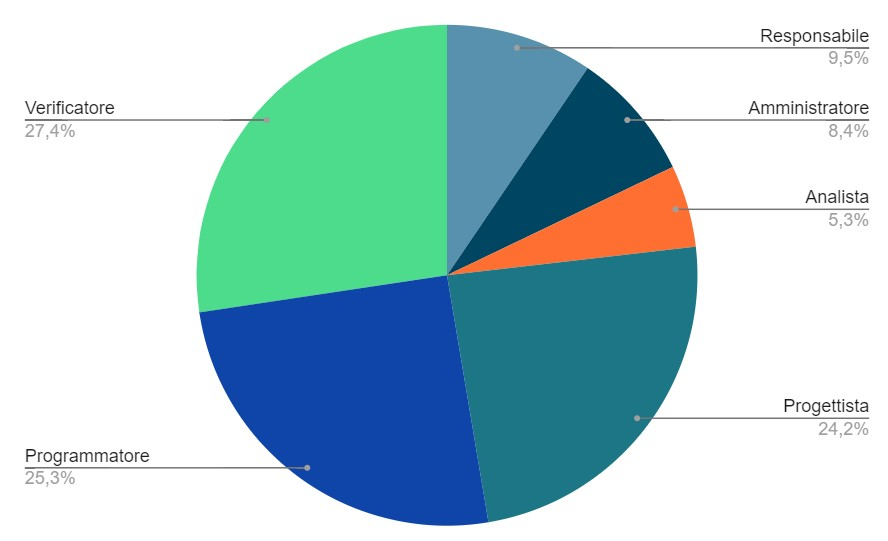
\includegraphics[width=1.0\textwidth]{percentuale_ore}
\end{center}

Il costo finale calcolato in base alle tariffe orarie dei ruoli e alle ore preventivate risulta di :
\textbf{€ 13160}.

In totale il monte ore è pari a \textbf{665 ore}, quindi \textbf{95 ore a testa} per ciascun membro del gruppo.
